Za potrebe provođenja eksperimenata preuzeli smo skup podataka iz repozitorija autora rada \cite{huang2024musicstyletransferdiffusion}. Skup se sastoji od 253 zvučnih zapisa .wav formata koji svaki traje po 5 sekundi. Zapisi su prikupljeni s web-stranice Pixabay te podijeljeni na zapise sadržaja (engl. \textit{content}) i zapise stila (engl. \textit{style}). Nakon podjele, skup podataka sadrži ukupno 179 zapisa sadržaja te 74 zapisa stila. Zapisi sadržaja podijeljeni su u 13 različitih kategorija, dok su zapisi stila podijeljeni na 18 različitih stilova. Pojedini zapisi obuhvaćaju širok spektar instrumenata i stilova kako bismo što podrobnije ispitali kapacitet i uspješnost našeg modela.

Glavna ideja našeg pristupa jest da se model nauči na zvučnim zapisima odabranog stila, npr. \textit{harmonica}, te da se naučeni stil potom prenosi na željene zapise sadržaja.

U svrhu obrade zvučnih podataka koristit ćemo podatkovnu reprezentaciju zvanu mel-spektrogram. Mel-spektrogram služi za vizualni prikaz frekvencijskog sadržaja zvuka u vremenu. Frekvencije na spektrogramu prilagođene su na takozvanu mel skalu koja odgovara ljudskom doživljaju odnosa među pojedinim tonovima. Takvi nam spektrogrami odgovaraju jer omogućuju jednostavan prikaz zvukova u domeni ljudske percepcije. Dodatno, njima možemo izravno manipulirati tijekom postupka prenošenja stila koristeći modele koji rade sa slikama. Kako bismo pretvorili zvučni zapis .wav formata u mel-spektrogram, koristimo \textit{Short Time Fourier Transform} (STFT). Nakon prenošenja stila, dobivene izmijenjene mel-spektrograme pretvaramo natrag u zvučne zapise pomoću Griffin-Lim algoritma.

\begin{figure}[H]
    \centering
    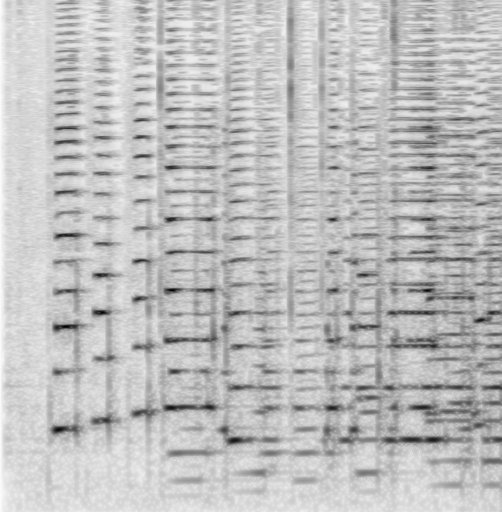
\includegraphics[width=0.5\linewidth]{imgs/spektrogram.png}
    \caption{Primjer jednog mel-spektrograma}
    \label{fig:spektrogram_primjer}
\end{figure}